\chapter{Part 2: Prediction of Monsoon Onset}
\label{c:part2}
As we have already seen, the onset of the ISM plays a very important role in the daily lives of the Indian population as well as the Indian economy overall.

[TODO: further intro]

\section{The ERA-Interim Dataset}
\label{st:era_interim}
[TODO: describe ERA-Interim same as TRMM has been described]

\begin{table}[h]
  \centering
  \begin{tabular}{|r|l|}
    \hline
    \textbf{ID} & \textbf{Description} \\
    \hline
    \textbf{msl} & Mean-Sea Level Pressure \\
    \textbf{r} & Relative Humidity at 1000hPa \\
    \textbf{t} & Temperature at 1000hPa \\
    \textbf{u700} & U-Component of Wind at 700hPa \\
    \textbf{v700} & V-Component of Wind at 700hPa \\
    \textbf{u200} & U-Component of Wind at 200hPa \\
    \hline
  \end{tabular}
  \caption{List of features from ERA-Interim that are used in this work.}
  \label{tab:era_features}
\end{table}

\section{Related Work}
[TODO: filler]

\subsection{Prediction of monsoon onset and variability}
\label{sst:related_prediction}
[TODO: ? describe other methods that have been proposed for onset prediction?]

[TODO: ? describe deep learning methods that have been used for precipitation prediction?]

% Due to the large number of factors at play, the exact determination and accurate prediction of monsoon onset dates for different parts of India is a challenging task. The IMD is the official Indian agency that observes and predicts the behavior of monsoon and tries to determine such accurate onset dates \citep{Pradhan.2017}...

\subsection{Neural networks}
\label{sst:neural_networks}
Many of our experimental models are based on a relatively new approach to training neural networks on spatio-temporal data. We specifically refer to the work of \citet{Shi.2015}, where a newly defined \textit{ConvLSTM2D} neural network layer was first applied to precipitation forecasting. Due to the reliance of many of our models on these layers, this section is thought to provide an intuition about their inner workings.

We generally assume that the reader is at least familiar with basic neural network principles for the remainder of this work. However, as convolutional and recurrent layers are what ConvLSTM2D layers are based on, we first shortly summarize the respective characteristics of these types of layers. We then go into the specific work of \citet{Shi.2015} and their approach to creating the convolutional recurrent ConvLSTM2D layer and describe the areas where their approach has already been tried.

\subsubsection{Convolutional neural networks}
\label{ssst:convolutional_networks}
[TODO: ? basics of conv nets (probably based on goodfellow "deep learning")?]

\subsubsection{Recurrent neural networks}
\label{ssst:recurrent_networks}
[TODO: ? basics of recurrent nets (probably based on goodfellow "deep learning")?]

\subsubsection{ConvLSTM2D}
\label{ssst:conv_lstm_2d}
[TODO: basics of conv recurrent nets based on the ConvLSTM2D paper]


\newpage
\section{Prediction of Monsoon Onset using Neural Networks}
\label{st:nn_implementation}
Looking to find a model capable of learning the patterns leading up to the monsoon onset, as well as predicting the onset itself, we have evaluated many different approaches to training neural networks based on spatiotemporal datasets like TRMM and ERA-Interim. Each approach had its own advantages and disadvantages, many of which we only learned through trial and error and subsequently used to build an improved architecture. Over many iterations with vastly different model architectures, we have finally gotten to a model that seems to be able to learn patterns present before the monsoon onset and, based on these patterns, predict the monsoon onset with reasonable accuracy.

The first part of this section is thus focused on our certainly most important and useful result: our final working models and their evaluation. We describe their general architecture as well as the different evaluation schemes and parameters we have used. Furthermore, we evaluate how well the models have performed over all our experiments and assess the prediction capabilities from different points of view (e.g., how accurately can we predict on the 15th of May, or how accurately can we predict 10 days before onset).

That being said, we would probably not have gotten to our final models without having tried many other architectures beforehand, iteratively improving upon the findings of each. The remainder of this section is therefore dedicated to a brief overview over all the model architectures we have evaluated during the creation of this work (in chronological order), along with a summary of our most important findings and results during the process.

\subsection{E4: A working model based on ERA-Interim}
\label{sst:final_model}
The neural network architectures and hyperparameter tunings that we have found to work best during the course of our experiments are based on two main ingredients: the ERA-Interim dataset with several of its features and multiple stacked convolutional recurrent layers (ConvLSTM2D). We have already introduced these

Our models are all based on the latest Keras 2.0 and Tensorflow 1.4 Python libraries, which have greatly simplified the creation of our models. At its core, Keras already includes ConvLSTM2D functionality (along with an appropriate default tuning), which meant that we did not need to implement any layers ourselves (be it in Keras or Tensorflow).

[TODO: extend]

\subsubsection{Data preprocessing}
One of the most important parts during the process of creating a neural network model (or any other machine learning model at that) is the preparation of the data that is to be used as its foundation. Without properly formatted input data, a neural network will typically not be able to learn any meaningful patterns. Over the course of our experiments, we have tried different datasets (TRMM and ERA-Interim) and, more importantly, many heterogenous input formats, of which each had its own advantages and disadvantages (we go over all of these evaluated input formats in their respective sections).

The approach we use in our final model architecture is most easily explained by means of an example: given time series data before the monsoon onset in an arbitrary year, we extract a fixed-length sequence (for example, a sequence of 60 subsequent days). The sequence ends at a given distance before the onset (e.g., 14 days before) and starts 60 more days before that. Feeding this sequence (corresponding to a single training example) to our neural network model after training, we would like it to predict the number 14, which is comparable to a simple regression task. Intuitively, we ask our model the following question: "given the last 60 days, in how many days from today will the monsoon arrive?".

If we were to train our model only based on sequences that end 14 days before the onset, it would most certainly always predict the number 14, no matter the actual input. To train our model for different distances, we need to repeat the sequence extraction process many times per year, using a different distance to the monsoon onset in each repetition. Our most successful models are based on 30 training examples per year with distances in the range of $[1, 30]$ and a sequence length of around 2 months.

The actual preprocessing of the ERA-Interim dataset is only slightly more complex: instead of a simple time series, from which a sequence is extracted, we have a time series where each timestep is represented by a multidimensional matrix (a \textit{3D-tensor}). For each location in the ERA-Interim coordinate grid as well as for each feature used from ERA-Interim (e.g., temperature), these tensors contain the value of the respective feature at the respective location (at that timestep). This is more intuitively shown in \cref{fig:e4_preprocessing}.

\begin{figure}[h]
  \centering
  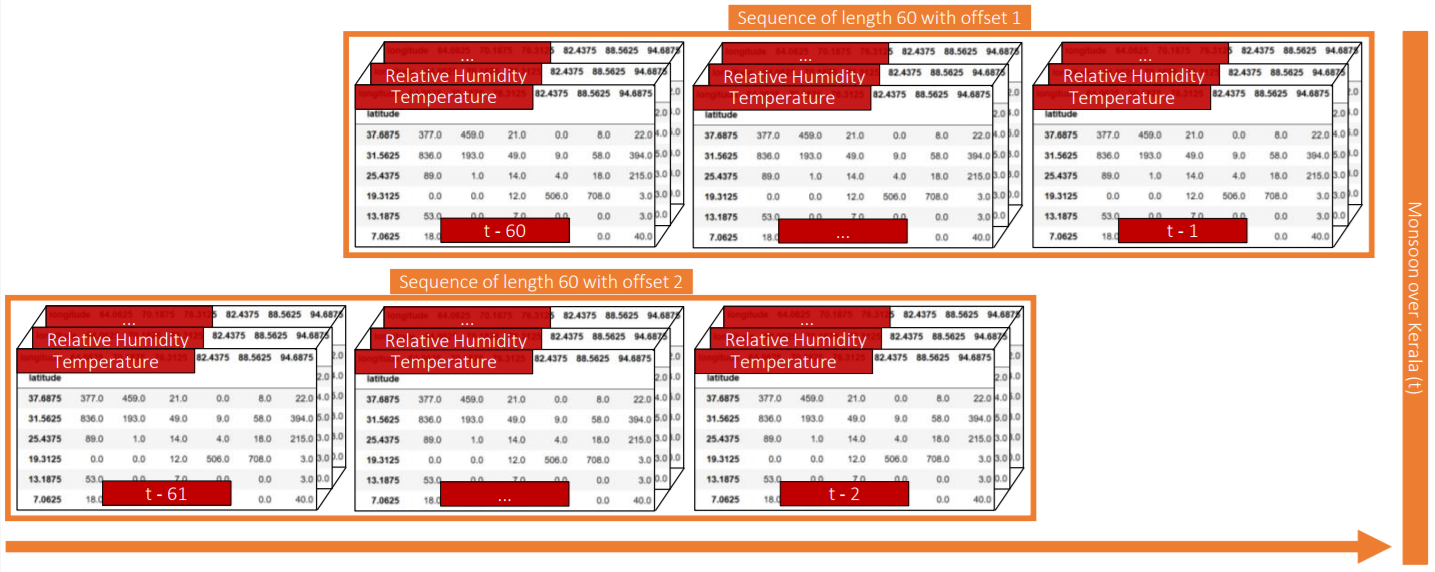
\includegraphics[width=\linewidth]{./99_appendix/img/E4_preprocessing}
  \caption{Data preprocessing for models of the E4 class.}
  \label{fig:e4_preprocessing}
\end{figure}

\paragraph{Normalization} An additional step during data preprocessing is often the normalization of data into certain consistent ranges. Even though neural networks could learn without normalization, it often improves and speeds up their learning process. If different input features clearly do not adhere to the same distribution (e.g., temperature and rainfall), the different magnitudes can lead to problems during the optimization process (when multiplying with the learning rate). When processing the ERA-Interim dataset into a training, validation and test set, we therefore apply statistical standardization to center the mean of each feature seperately. To prevent the introduction of any bias, the mean and standard deviation of the training set are reused when normalizing the validation and test sets.

\clearpage
\subsubsection{Model architecture}
It is not hard to see that a single ERA-Interim coordinate grid is inherently similar to a simple multichannel image: we have a height (latitudes), a width (longitudes) and multiple channels (e.g., temperature and relative humidity). When working with images, convolutional neural networks are by far the most prevalent approach, having led to great progress in image recognition and other domains. However, 2D-convolutions are not directly applicable to multiple images ordered in a sequence (like a movie). Instead, they first need to be combined with recurrent network structures like LSTM.

We have already introduced a recent approach to the problem of learning from spatiotemporal data: the ConvLSTM2D neural network layer (\cref{ssst:conv_lstm_2d}). In our case, this layer performed much better than a simple stacking of convolutional and recurrent layers, making it the most important part in many of our models (including E4). With ConvLSTM2D at its core, the E4 model architecture performs a regression by flattening the final output of the ConvLSTM2D layers and passing it through multiple dense layers, the final one of which has only a single neuron (and thus yields a single number). As an optional addition, time-distributed convolutional and pooling layers can be applied before passing the sequence into the ConvLSTM2D layers, adding further feature detection and dimensionality reduction capabilities. An exemplary model based on the described architecture is shown in \cref{fig:e4_architecture}.

\begin{figure}[h]
  \centering
  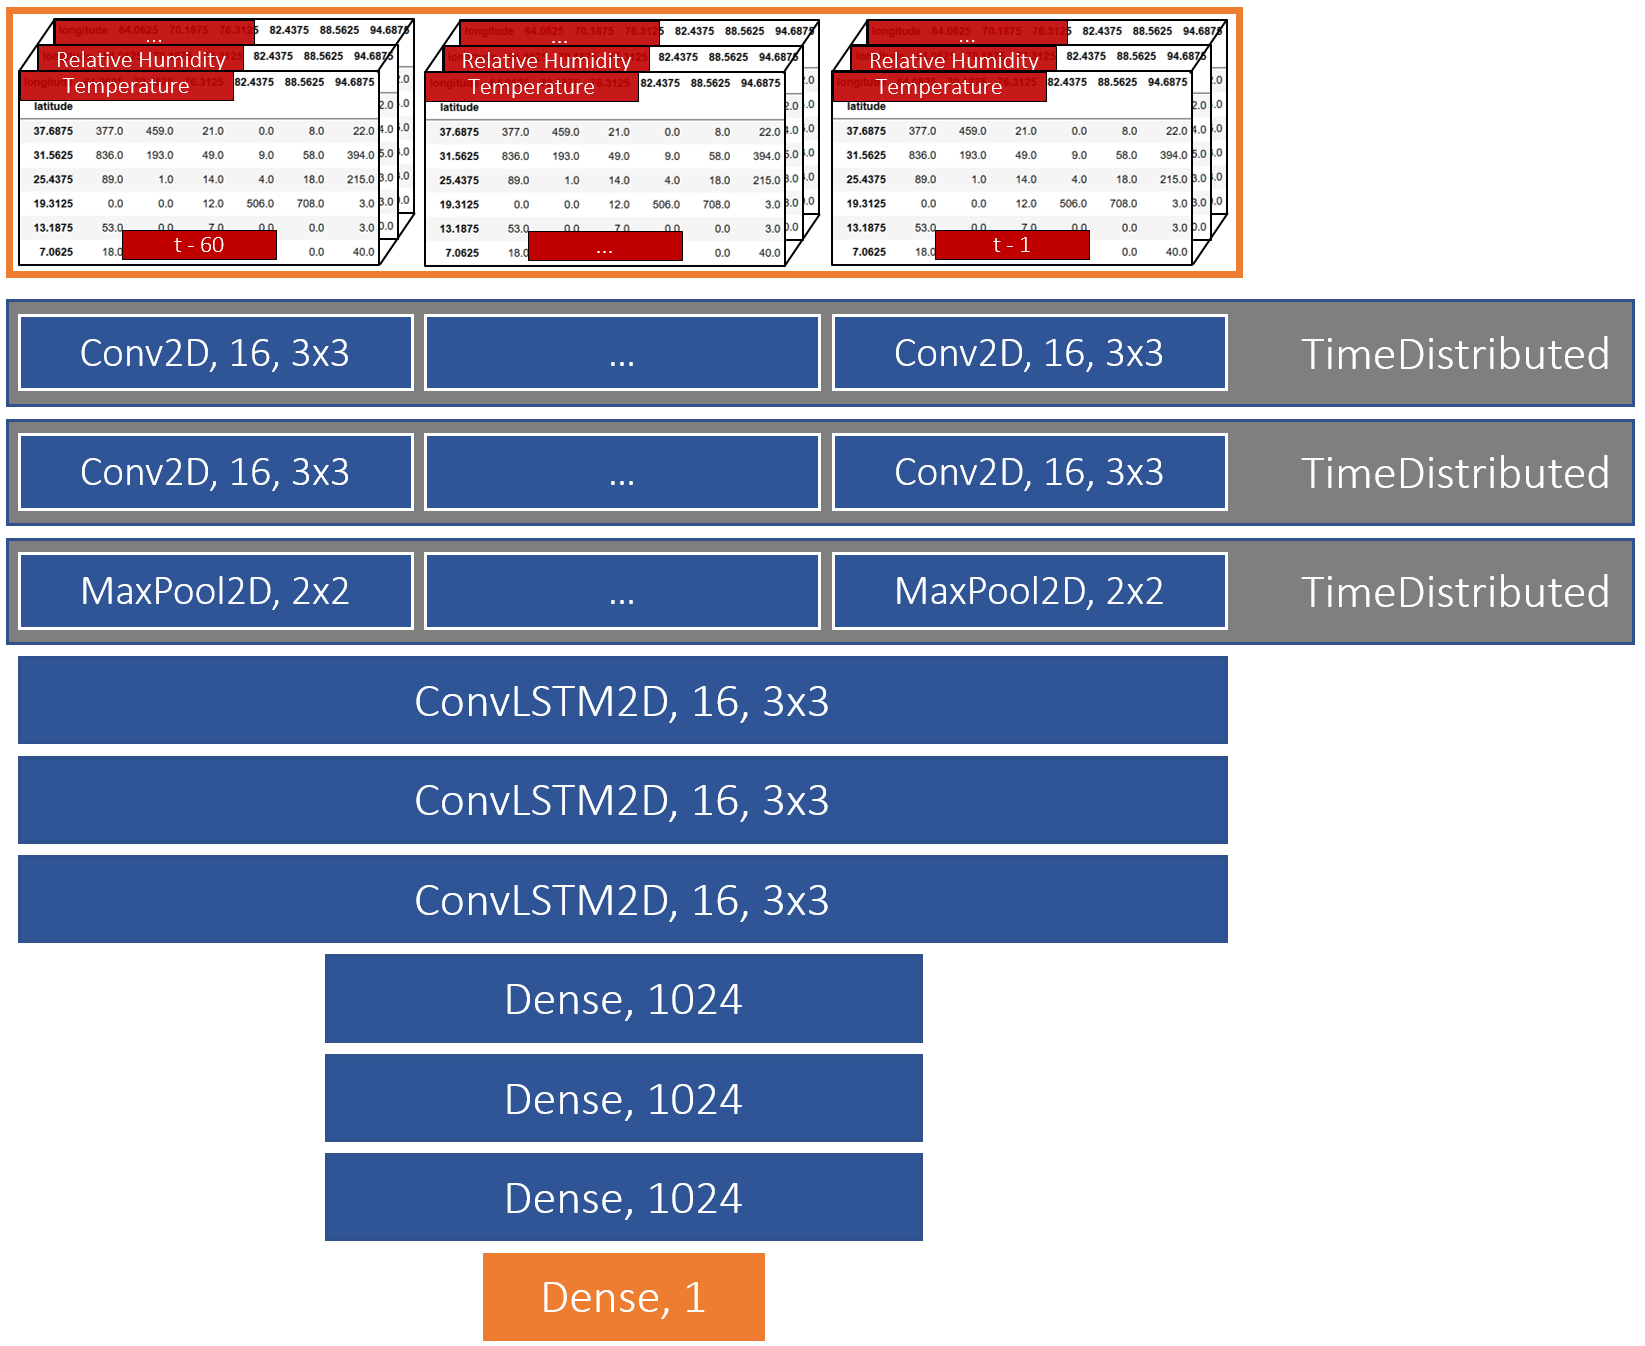
\includegraphics[width=0.8\linewidth]{./99_appendix/img/E4_architecture}
  \caption{Exemplary model architecture of the E4 class.}
  \label{fig:e4_architecture}
\end{figure}

\paragraph{Regularization} To reduce the tendency of the model to overfit to the training set, we apply L2-regularization to the kernels of all types of layers (Conv2D, ConvLSTM2D, Dense). This increases the loss whenever the model's internal representation of the problem gets too complex, effectively improving its ability to generalize. In addition, we can and do most often use dropout after each layer. However, the exact regularization and dropout parameters vary with each tuning.


\subsubsection{Model evaluation}
On our search for the best configuration to train our models with, we have performed 45 experiments for this final model architecture alone. The parameter space we were searching through can be split into two major categories: ``hyperparameters'', referring to the parameters that are typically heavily tuned to improve model performance (e.g., learning rate, dropout rates, kernel sizes, etc.), and a second category that is more fundamental, as it already influences the data when it is being preprocessed. The choice of datasets and features thereof, as well as the amount of data that is being fed to the model (e.g., the sequence length), are exemplary parameters that we assign to the latter category. An overview of such ``meta-hyperparameters'' is shown in \cref{tab:meta_parameters}.

\begin{table}[h]
  \centering
  \begin{tabular}{|r|c|c|c|c|c|c|}
    \hline
    \textbf{ERA-Features} & \multicolumn{2}{c|}{msl/r/t} & \multicolumn{2}{c|}{msl/r/t/u700/v700} & \multicolumn{2}{c|}{msl/r/t/u700/v700/u200} \\
    \hline
    \textbf{Onset Dates} & \multicolumn{3}{c|}{IMD (1979-2017)} & \multicolumn{3}{c|}{Objective (1979-2007) + IMD (2007-2017)} \\
    \hline
    \textbf{Sequence Length} & 32 & 42 & 47 & 62 & 77 & 92 \\
    \hline
    \textbf{Sequence Offset} & 0-8 & 0-21 & 0-22 & 5-25 & 0-30 & 1-30 \\
    \hline
  \end{tabular}
  \caption{``Meta-hyperparameters'' as they have been used in the final E4-class models. IMD onset dates until 2007 are extracted from \citet{Singh.2009} and concatenated with official IMD dates (2007-2017). Objective onset dates are extracted from the same source, but then also concatenated with IMD dates. The Sequence Offset specifies the range of offsets that is generated (meaning that for a value of 1-30, 30 examples are generated for each year). Details about the ERA-Features can be found in \cref{tab:era_features}. }
  \label{tab:meta_parameters}
\end{table}

\paragraph{Training, validation and test set}
The ERA-Interim dataset was split into three fixed sets for each of our experiments: a training, validation and test set. As can be seen in \cref{tab:train_test_split}, we originally started with only 3 years in the validation and 5 years in the test set (out of 38 years). When many models seemed to fit to the training set very well, we decided to reduce the size of the training set, extending both the validation and test set (to 4 and 8 years, respectively).

Due to the fact that the ``objective'' onset dates stem from two different distributions (data that follows the objective definition is available until 2007, after which the dates come from the IMD), model performance was much worse when using the second split. After it was reduced to the years 1979-2005, the training set did no longer contain years based on the official IMD dates, while most of the validation and test set were based on these IMD dates. Unsurprisingly, the overall strongest overfitting was observed in the few experiments that were carried out this way. As a remedy to this problem, we devised a third split scheme with a more appropriate distribution of years, which was then used successfully for the remainder of the experiments.

It needs to be noted that tuning models on one split scheme and changing this scheme afterwards could introduce bias, as years that the model might have trained on in a previous experiment could suddenly belong to the test set. It cannot be completely disqualified that some bias might be present in our later models due to these changes, even though we took care to introduce the least possible of it. It is generally best to devise one split scheme and apply this scheme to all experiments.

\begin{table}[h]
  \centering
  \begin{tabular}{|r|c|c|c|}
    \hline
    & \textbf{Split 1} & \textbf{Split 2} & \textbf{Split 3} \\
    \hline
    \textbf{Validation} & 2010-2012 & 2006-2009 & 80/90/00/10/16 \\
    \textbf{Test} & 2013-2017 & 2010-2017 & 85/95/03/04/05/14/15/17 \\
    \hline
    \textbf{Experiments} & 0-27 & 28-31 & 32-45 \\
    \hline
  \end{tabular}
  \caption{The three different splits that have been applied to the dataset in the experiments for E4.}
  \label{tab:train_test_split}
\end{table}

\paragraph{Evaluation schemes}
Over the course of our experiments, we have used various combinations of ``meta-hyperparameters'', leading to what can be called \textit{evaluation schemes}. An evaluation scheme is a group of experiments that are based on the same high-level parameters but have been tuned using different hyperparameters. We can reduce the total of our 45 experiments to 17 such evaluation schemes, each consisting of one to nine experiments. The listing in \cref{tab:evaluation_schemes} shows these 17 evaluation schemes along with their configuration.

\begin{table}[h]
  \centering
  \begin{tabular}{|r|c|c|c|c|c|}
    \hline
    \textbf{ID} & \textbf{ERA-Features} & \textbf{Onset Dates} & \textbf{Seq. Length} & \textbf{Seq. Offset}  & \textbf{\#} \\
    \hline
    EV01 & msl/r/t & IMD & 47 & 1-30 & 1 \\
    \hline
    EV02 & msl/r/t & IMD & 62 & 1-30 & 2 \\
    \hline
    EV03 & msl/r/t & IMD & 77 & 1-30 & 1 \\
    \hline
    EV04 & msl/r/t & Objective+IMD & 62 & 5-25 & 3 \\
    \hline
    EV05 & msl/r/t & Objective+IMD & 62 & 0-30 & 3 \\
    \hline
    EV06 & msl/r/t & Objective+IMD & 62 & 1-30 & 3 \\
    \hline
    EV07 & msl/r/t/u700/v700 & IMD & 62 & 1-30 & 9 \\
    \hline
    EV08 & msl/r/t/u700/v700 & Objective+IMD & 32 & 0-30 & 1 \\
    \hline
    EV09 & msl/r/t/u700/v700 & Objective+IMD & 62 & 0-21 & 3 \\
    \hline
    EV10 & msl/r/t/u700/v700 & Objective+IMD & 62 & 0-22 & 8 \\
    \hline
    EV11 & msl/r/t/u700/v700 & Objective+IMD & 62 & 0-30 & 3 \\
    \hline
    EV12 & msl/r/t/u700/v700 & Objective+IMD & 62 & 1-30 & 2 \\
    \hline
    EV13 & msl/r/t/u700/v700 & Objective+IMD & 62 & 0-8 & 3 \\
    \hline
    EV14 & msl/r/t/u700/v700 & Objective+IMD & 92 & 0-30 & 1 \\
    \hline
    EV15 & msl/r/t/u700/v700/u200 & Objective+IMD & 42 & 0-30 & 1 \\
    \hline
    EV16 & msl/r/t/u700/v700/u200 & Objective+IMD & 62 & 0-30 & 1 \\
    \hline
    \multicolumn{5}{|r|}{\textbf{TOTAL}} & 45 \\
    \hline
  \end{tabular}
  \caption{Evaluation schemes for the E4-class models and the corresponding number of experiments, based on the ``meta-hyperparameters'' as shown in \cref{tab:meta_parameters}. Details about the ERA-features can be found in \cref{tab:era_features}}
  \label{tab:evaluation_schemes}
\end{table}

Based on the evaluation schemes we have previously defined,


\begin{table}[h]
  \centering
  \begin{tabular}{|r|c|c|c|c|}
    \hline
    \textbf{ID} & \textbf{10 epochs} & \textbf{30 epochs} & \textbf{50 epochs} & \textbf{100 epochs} & & \textbf{Final epoch} \\
    \hline
    EV1 & 48/132 & 37/85 & 30/87 & 15/72 & 11/68 (500) \\
    \hline
    EVx &  &  &  &  &  \\
    \hline
    EVx &  &  &  &  &  \\
    \hline

    \hline
  \end{tabular}
  \caption{Easdf}
  \label{tab:evaluation_scheme_results}
\end{table}



Based on the

\subsection{T1-T5 and E1-E3: Other model architectures}
blabla


we have evaluated many different neural network architectures and tunings during the creation of this work. This section provides a high-level overview of these architectures


This section walks through the different variations of neural network models we have evaluated during the creation of this work. The variations can differ in their network structure, in the data and features used to train the model or simply in the tuning of hyperparameters applied. \cref{tab:nn_overall_summary} summarizes the key characteristics of all models we have built and evaluated.

Each model architecture is further associated a unique version identifier that we will use when referring to the specific architecture. The identifiers are based on the type of dataset used to train the model and the variation of the model architecture used (e.g., \textit{T1}: TRMM v1, \textit{E3}: ERA-Interim v3, \textit{TE1}: TRMM and ERA-Interim v1). All of the models presented were built and trained using the latest Keras 2.0 and Tensorflow 1.3/1.4 libraries for Python.

[TODO: extend]

\begin{table}[h]
  \begin{tabularx}{\linewidth}{|c|X|}
    \hline
    Model & Architectural Key Points \\
    \hline
    T1 & First trials with LSTM and TRMM; No experiments; Discarded \\
    T2 & Each location of each year as a separate example; Sequences of values for single grid cells processed with LSTM; Categorical prediction on the 11th of May (predicted MoK in 1-40 days) \\
    T3 & Each year as a separate example; One sequence of TRMM grids (daily values) per year processed with ConvLSTM2D; Numerical prediction on the 11th of May (predicted MoK in x days) \\
    T4 & Regularization for dense, convolutional and recurrent layers; Based on T3 \\
    T5 & Objective or IMD onset dates from \citep{Singh.2009}; Prediction on the 22nd of May; Based on E2 \\
    \hline
    E1 & Training on the ERA-Interim dataset and multiple features (temperature, relative humidity); Based on T4 \\
    E2 & Objective or IMD onset dates from \citep{Singh.2009}; Prediction on the 22nd of May; Based on E1 \\
    E3 & Improved structuring of Python classes; Extraction of core model logic into base classes; Same functionality as E2; No experiments \\
    E4 & Multiple examples per year with variable offset to the onset date; Choice of additional input features; Possibility for additional 2D-convolutions before ConvLSTM2D; Switch to the functional Keras API; Based on E3 \\
    \hline
  \end{tabularx}
  \caption{Overview of all neural network models that have been built \& evaluated}
  \label{tab:nn_overall_summary}
\end{table}



\newpage
\subsection{T2: Naive classification models using TRMM}
\label{sst:nn_t2}
The first models we evaluated were classification networks based on the TRMM dataset (see \cref{sst:trmm_dataset}) at various spatial resolutions (ranging from a 0.25\degree x 0.25\degree resolution to an aggregated 2.5\degree x 2.5\degree resolution). This chapter briefly describes the structure of these first models.

\subsubsection{Data preprocessing}
\label{ssst:nn_t2_data}
A single TRMM cell (i.e., a single location on the grid) was taken at a time and transformed into a time series for that specific location (from the first of May up to the prediction date). The latitude and longitude indices were appended in front of the time series to allow the network to learn the spatial features of each example. This led to training examples each consisting of a one-dimensional fixed-length sequence containing coordinates and daily rainfall amounts as well as a label corresponding to its category. \cref{tab:nn_t2_data} provides an overview about the structure of the examples used to train and evaluate the model.

The labels were represented as one-hot encoded vectors like $\left[ 0, ..., 1, ..., 0 \right]$. They were calculated based on the difference in days between the fixed prediction date and the monsoon onset date over Kerala. As the earliest onset in [Onset Dates v1] for the relevant period (1998-2017) was found to be on the 12th of May, the prediction date was set to be the 11th of May. With the latest historical onset during the available period (1887-2017) being on the 15th of June, the category labels were naturally restricted to a range of $\left[ 1, 35 \right]$. Some additional padding was added to allow for future late onsets, yielding a range of $\left[ 1, 40 \right]$. Due to the focus on the onset date over Kerala, the examples for each year could all be assigned the label for the respective year.

\begin{table}[h]
  \centering
  \begin{tabular}{|ccrrrr||c|}
    \hline
    Latitude & Longitude & 01.03.1998 & 02.03.1998 & ... & 11.05.1998 & Label \\
    \hline
    \hline
    6.375 & 63.625 & 0.27 & 0.09 & ... & 3397.29 & [0, ..., 1, ..., 0] \\
    6.375 & 66.125 & 0.03 & 10.08 & ... & 4632.24 & [0, ..., 1, ..., 0] \\
    ... & ... & ... & ... & ... & ... & [0, ..., 1, ..., 0] \\
    36.375 & 91.125 & 0.79 & 0.00 & ... & 68.61 & [0, ..., 1, ..., 0] \\
    36.375 & 93.625 & 11.44 & 0.06 & ... & 40.06 & [0, ..., 1, ..., 0] \\
    \hline
  \end{tabular}
  \caption{Exemplary list of training examples for the year 1998 at 2.5\degree aggregation.}
  \label{tab:nn_t2_data}
\end{table}

\subsubsection{Modeling}
\label{ssst:nn_t2_model}
To build a model based on the preprocessed examples, a sequence of LSTM and Dense layers was trained on the training set. A final softmax layer allowed the prediction of classes. Losses were thereby calculated using categorical cross-entropy. A percentage of training data was randomly held out in each epoch to validate the intermediary results.

\begin{figure}[h]
  \centering
  [TODO: visualization]
\end{figure}

\begin{lstlisting}[language=Python]
  [TODO: pseudocode]
\end{lstlisting}

\subsubsection{Preliminary results}{\footnote{Exact results will be compared in between all models in the evaluation section (\cref{sst:nn_results})}}
\label{ssst:nn_t2_results}
The presented classification approach was soon discarded due to poor overall learning capabilities. Firstly, classification was found not to be a suitable approach for prediction of an upcoming onset date. An adequate loss should incorporate the numerical distance in days between the predicted and the true onset date, which is not easily possible when evaluating classification using cross-entropy loss. The implementation of a custom loss function could remediate some of these concerns but was not regarded as useful at the time.

Secondly, using each grid cell as a separate example might have led to a larger number of training examples overall, but rainfall in sepa rate single geographical locations in India probably cannot be seen as a reasonable predictor for a large-scale phenomenon like monsoon onset. It cannot be ensured that the model would be able to learn any spatial relationships based on the inclusion of coordinates as the very first timesteps in each sequence. As we have already explored in \cref{st:ism_factors}, the behavior of Indian Summer Monsoon is influenced by many external factors that are not necessarily restricted to the Indian subcontinent. Thus it is most probably a combination of many places (some of which more important than others) that could lead to successful onset date predictions.

A further disqualifying factor against the use of any such classification approach was the fact that the model would be unable to express any future onset occurring outside the borders of the classification (e.g., more than 40 days after the prediction date). As we have elaborated in \cref{st:ism_trends}, the behavior of the ISM is ever-changing and it cannot be ruled out that the onset date distribution will change significantly in the time to come.


\subsection{T3 \& T4: First convolutional models using TRMM}
\label{sst:nn_t3}
The findings of the first naive classification suggested that the overall model architecture and the data input shape needed to be rethought. To be able to capture temporal as well as spatial relationships between different geographical locations in India, the input time series needed to be changed such that each timestep would contain daily data for the entire Indian subcontinent.

\subsubsection{Data preprocessing}
\label{ssst:nn_t3_data}
To extend the dimensionality of the input data, the TRMM dataset was transformed to a fixed-length sequence of coordinate grids (each coordinate grid thereof containing data for all locations). This resulted in only a single training example per year of data. As TRMM data is available from 1998 onwards and with some data that would be held out for validation and testing, the number of training examples shrunk to roughly a dozen.

Furthermore, keeping the outcome calculations the same as for the previous classification task, the classification was changed to numerical regression. Instead of trying to predict one of the classes in the range $\left[ 1, 40 \right]$, the model would thus predict an exact number that could be both higher or lower than numbers in the classification range. However, the prediction would still represent the predicted number of days from the prediction date until the occurrence of monsoon onset over Kerala.

\begin{table}[h]
  \centering
  \begin{tabular}{|r||rrrrr|}
    \hline
    Lat./Lon. & 63.375 & 64.375 & ... & 95.375 & 96.375 \\
    \hline
    \hline
    6.125 & 849.779974 & 791.189987 & ... & 139.547018 & 430.566095 \\
    7.125 & 323.249996 & 393.899986 & ... & 38.789999 & 172.289993 \\
    ... & ... & ... & ... & ... & ...\\
    38.125 & 0.000000 & 0.000000 & ... & 1.648755 & 7.281448 \\
    39.125 & 0.000000 & 0.000000 & ... & 1.584739 & 1.154755 \\
    \hline
  \end{tabular}
  \caption{An exemplary coordinate grid aggregated to 1.0\degree. A sequence of 72 such matrices and its label correspond to a full training example (one year of data).}
  \label{tab:nn_t3_data}
\end{table}

\subsubsection{Modeling}
\label{ssst:nn_t3_model}
To be able to process a sequence of grids (i.e., matrices), the first layers of the model needed to be able to handle multi-dimensional input sequences. These layers were therefore changed from a regular LSTM layer to Convolutional LSTM layers (see \cref{sst:conv_recurrent_networks} on ConvLSTM2D layers). These layers can process a sequence of multi-dimensional input matrices and learn complex spatial as well as temporal relationships.

The new model architecture (T3) further included batch normalization to improve training speed. In comparison to the previously used cross-entropy loss, mean-squared or mean-absolute error could now provide a reasonable distance metric.

A later extension (T4) added regularization for the convolutional, recurrent and dense layers to improve the models' ability to generalize. Furthermore, the validation set was changed from a random percentage of the training set to a fixed set of years. The validation years were defined to be the latest in the training set such that long-term trends could be captured by the model, which might not have been possible using the previous random validation split.

\begin{figure}[h]
  \centering
  [TODO: visualization]
\end{figure}

\begin{lstlisting}[language=Python]
  [TODO: pseudocode]
\end{lstlisting}

\subsubsection{Preliminary results}{\footnote{Exact results will be compared in between all models in the evaluation section (\cref{sst:nn_results})}}
\label{ssst:nn_t3_results}
Many experiments with various hyperparameter tunings showed that the first variation of the model architecture (T3) was unable to fully learn the concepts of the training set and that it did not generalize to the validation set very well.

The results of experiments for the T4 variation were much improved, especially if regularization was used for all types of layers (in addition to dropout). In training, the model converged up to a certain point but tended to plateau afterward, even if run for hundreds of epochs. This would normally suggest that the optimization process has reached either a minimum or is otherwise unable to learn any further, except that in this case, the validation loss plateaued as well (instead of increasing due to a growing tendency to overfit).

\begin{figure}[h]
  \centering
  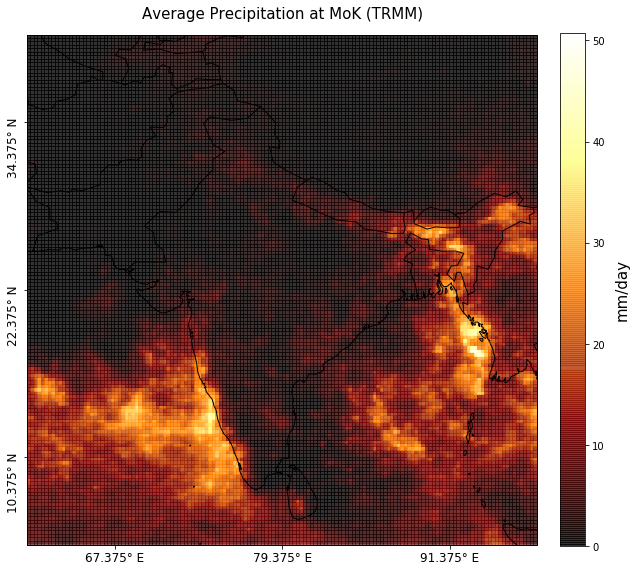
\includegraphics[width=0.4\linewidth]{./99_appendix/img/prec_avg_onset}
  \caption{Average precipitation at MoK (TRMM, 1998-2017)}
  \label{fig:trmm_prec_onset}
\end{figure}

We found that, in this case, the models learned a way to get close to the real outcomes without learning anything about the patterns in the input data: all the outcomes of the validation and test sets were simply predicted to be the mean value of the outcomes in the training set. There could be several explanations for this behavior, but many suggest that something is off with the input data. It might be that the sparsity of the TRMM dataset (as visualized in \cref{fig:trmm_prec_onset}) and its many places without any rainfall prevent the neural network from learning any useful patterns. Alternatively, it could be that we are trying to find patterns in the input data that don't exist in the way we would have imagined (i.e., that we are trying to fit a model to noise).


\subsection{E1: Convolutional models using ERA-Interim}
\label{sst:nn_e1}
The overall results from T1 up to T4 suggested that the TRMM dataset on its own might not be well suited for the prediction task at hand. An obvious way of improvement was to use another dataset for the prediction tasks, namely the ERA-Interim reanalysis dataset.

Compared to the TRMM dataset, the ERA-Interim dataset brings with it several advantages relevant to our task. Firstly, much more data is available (dating back to 1979 instead of 1998), which can improve the performance of deep neural networks significantly (even though the number of total examples is still comparatively small). Secondly, there are many more features (of which some could prove to be better predictors than solely the amount of daily rainfall). Furthermore, the dataset had already been used for onset prediction tasks in \citep{Stolbova.2015}.

A disadvantage of using the ERA-Interim dataset might be that its spatial resolution is much lower than the one of the TRMM dataset (0.75\degree x 0.75\degree compared to 0.25\degree x 0.25\degree). When training with the ERA-Interim dataset, the input matrices in the sequence would thus be much smaller in the spatial dimensions (latitude and longitude), providing the models with less detailed data to train on. However, many more ERA-Interim features could be added as channels to the model inputs, giving the models the possibility to learn more complex patterns and relationships. The lower resolution of the ERA-Interim dataset further means that each input matrix is up to 9 times smaller than with TRMM, leading to lower overall computational effort and hardware requirements (i.e., memory capacity).

\subsubsection{Data preprocessing}
\label{ssst:nn_e1_data}
This first iteration of the ERA-based model (E1) made use of only two features from ERA-Interim: temperature and relative humidity each at a 1000hPa pressure level. [Stolbova] found this combination of features to be a reliable predictor of the monsoon onset date. While this finding should also apply to our problem, the approach used was based on statistical time-series analysis [TODO: oder so?] and as such might not directly transfer to the training of our neural network models.

To feed temperature and relative humidity to the model simulataneously, the features needed to be stacked in a single coordinate grid. Each grid cell would thus contain multiple channels (i.e. features, same as the RGB channels in images) and be represented as a 3D-tensor (i.e. a "3D matrix"). Combining grids to a sequence yielded a sequence of 3D-tensors (a 4D-tensor) that could then be used as input for the neural network models.

\subsubsection{Modeling}
\label{ssst:nn_e1_modeling}
Incorporating these findings into a new model structure, we extended the convolutional model to be able to learn from a sequence of 3D-tensors. The convolutional layers would then process these inputs just like they would process an RGB image with its three channels.

\begin{figure}[h]
  \centering
  [TODO: visualization]
\end{figure}

\begin{lstlisting}[language=Python]
  [TODO: pseudocode]
\end{lstlisting}

\subsubsection{Preliminary results}{\footnote{Exact results will be compared in between all models in the evaluation section (\cref{sst:nn_results})}}
\label{ssst:nn_e1_results}
Running experiments for the E1 model yielded results that displayed similar patterns to the TRMM-based models evaluated before: the models were learning up to a certain point and plateaued at unsatisfactory levels of loss and validation loss. They still seemed to get stuck during the learning process.

As experiments for entirely different datasets (TRMM and ERA) and many hyperparameter tunings for each showed similarly unsatisfactory patterns, it was probable that something was off with the data being fed into the model. Further research showed that the distribution of onset dates used seemed to show some irregularities that had not been regarded as irregular before: many onset dates were set in the first half of May (as early as on the 12th of May), which is highly improbable for typical ISM onsets\footnote{This was brought to light during consultation with V. Stolbova.}. These onset dates might, for example, have been caused by bogus monsoon onsets that were not registered as such at the time.

The labels of the training, validation and test examples were all calculated using the skewed onset dataset. The early outliers in the dataset forced us to predict even earlier, which is why predictions up to this point were always made on the 11th of May, and why the sequences were restricted to the 72 days in between 01.03-11.05 of each year.


\subsection{E2, E3 \& T5: Convolutional models with objective onset dates}
\label{sst:nn_e2t5}
After further analysis of onset distributions for different onset datasets, the objective definition of monsoon onset proposed by \citet{Singh.2009} seemed to be the most adequate for our training. The distribution seemed to be much less skewed overall, with more similarities to a uniform distribution than to a Gaussian normal distribution, at least when data was restricted to the relevant area between 1979-2017 (see \cref{apx:onset_dates} for the full analysis).

While it might be counterintuitive that the ISM onset would not follow a normal distribution (as many natural processes do), a more balanced distribution of labels can improve the performance of machine learning models. Many models work better if input data is preprocessed with stratification methods (i.e., classes are rebalanced), as the model might otherwise tend to predict the label that occurs most often in the training set.

Building on these findings, we then created the E2, E3 and T5 model versions, i.e., new models for both ERA-Interim and TRMM (as well as a combination of them) that were primarily a repetition of the best previous experiments with updated labels for the new onset dates.

\subsubsection{Data preprocessing}
\label{ssst:nn_e2t5_data}
Due to the new distribution of onset dates, the prediction date was newly set on the 22nd of May, increasing the available sequence length by 11 days (up to 83 days)...

[TODO: extend?]

\subsubsection{Modeling}
\label{ssst:nn_e2t5_modeling}
The models were not much changed, as they were already flexible enough to accept arbitrary sequence lengths and an arbitrary number of stacked features (channels)...

[TODO: extend?]

\begin{figure}[h]
  \centering
  [TODO: visualization]
\end{figure}

\begin{lstlisting}[language=Python]
  [TODO: pseudocode]
\end{lstlisting}

\subsubsection{Preliminary results}{\footnote{Exact results will be compared in between all models in the evaluation section (\cref{sst:nn_results})}}
\label{ssst:nn_e2t5_results}
Running the experiments for E2 and T5 yielded much better final losses. The validation loss could get as close as 2.5 days (TRMM) and 4.7 days (ERA) of mean-absolute error, which would suggest that T5 could predict the monsoon onset on the 22nd of May and do so with an accuracy of +- 2.5 days, which would have been a good result.

However, close examination of the actual predictions of the model was not as reassuring, as the model still seemed to predict only one single number for any validation or test example that was fed into the model. Furthermore, a combination of the TRMM and ERA dataset by stacking the three features yielded comparable results: the model again seemed to resort to predicting the mean of onsets based on the TRMM dataset.


\subsection{E4: Increasing the amount of training data}
\label{sst:nn_e4}
Following the bad generalization capabilities of all models up to their latest versions, an improvement to the overall training approach was sought. Up to versions E3 and T5, the dates of prediction were always fixed to a single date during the pre-monsoon period (22nd of May). This meant that for each year of data, only a single sequence could be extracted and used as a training example.

The patterns during the pre-monsoon period might not be conclusive enough to allow a model to predict future onsets reliably. Some patterns might be closely tied to a temporal distance to the monsoon onset, i.e., some event might always happen approximately two weeks before onset. This would have been captured by the model at different steps in the sequence, which could, in turn, have been suitable for prediction. On the other hand, the model might have missed many of these events because the data was cut off at the prediction date, possibly multiple weeks before the real onset date.

\begin{table}[h]
  \centering
  \begin{tabular}{ |c|c|c| }
    \hline
    head1 & head2 & head3 \\
    \hline
    cell1 & cell2 & cell3 \\
    \hline
  \end{tabular}
  \caption{TODO: summary table (validation years etc.)}
  \label{tab:nn_e4_summary}
\end{table}

\subsubsection{Data preprocessing}
\label{ssst:nn_e4_data}
To allow the model to capture all the events leading up to the onset of each respective year, the approach to training the model needed to be changed. Firstly, the model needed to be fed sequences with equal distances to the respective real onset date. For example, with an onset on the 10th of June, the sequence to be fed to the model could include data from the 9th of May to the 9th of June. Repeating this for each year in the training set while keeping a one-day distance to the real onset date and the length of the sequences fixed, the model should learn to predict that the onset will take place in exactly one day.

This would not be that useful by itself, as the model would then only be able to predict the onset one day in advance. However, this approach to training allows feeding the model multiple sequences per year, each with a different offset to the onset date and a correspondingly different label. The amount of available examples is as such greatly increased: generating three such sequences per year would triple the overall number of examples available for training. Furthermore, the prediction capabilities of the model could then be evaluated seperately for each offset, yielding results on how well the model can predict one day in advance, one week in advance or even multiple weeks in advance.

\subsubsection{Modeling}
\label{ssst:nn_e4_modeling}
As the model was already based on fixed-length sequences of grids, not much needed to be changed in the model architecture to allow for the new training approach.

[TODO: extend]

\begin{figure}[h]
  \centering
  [TODO: visualization]
\end{figure}

\begin{lstlisting}[language=Python]
  [TODO: pseudocode]
\end{lstlisting}

\subsubsection{Preliminary results}{\footnote{Exact results will be compared in between all models in the evaluation section (\cref{sst:nn_results})}}
\label{ssst:nn_e4_results}
[TODO: update once final experiments have run]


\clearpage
\subsection{Evaluation}
\label{sst:nn_results}
This section lists and subsequently compares the results of the many experiments performed using the models in this chapter. We focus on training and validation loss for the majority of experiments, as not all experiments were evaluated on the test set (in order to prevent tuning any of the models to the test set). We additionally show the test set performance for the best performing models of each version.

\subsubsection{Experimental conditions}
\label{ssst:experimental_conditions}
The experiments were run in different environments and are explicitly marked as such: either on a local GPU, on the IFI Kraken cluster or on a Paperspace\footnote{https://www.paperspace.com/} virtual machine. \cref{tab:experimental_environments} provides a more detailed overview of the environments used during the experimental phase.

\begin{table}[h]
  \centering
  \begin{tabular}{ |c|c|c| }
    \hline
    Environment & Trained on & Available Memory \\
    \hline
    Kraken & CPU (24-cores) & 128GB RAM \\
    Local & GPU (GTX 970) & 32GB RAM, 4GB GPU \\
    Paperspace & GPU (Quadro P5000) & 30GB RAM, 16GB GPU \\
    \hline
  \end{tabular}
  \caption{Runtime environments for the deep learning experiments.}
\label{tab:experimental_environments}
\end{table}

Depending on the model version and other experimental conditions (aggregation of input data, number of features, number of sequences per year, etc.), the preprocessed input data can take up many gigabytes of RAM. Many combinations were not possible to run on the local GPU due to the comparatively low GPU-memory constraint. This was true especially when processing the raw, unaggregated dataset.

The nodes of the Kraken cluster worked well for most of the experiments, especially when the 24 available cores were used exclusively for the training of a single model. However, it was still comparatively slow, and we were rarely able to run much more than 100 epochs in a 12h timeframe, for some model versions and types not even more than 50. Even when using up to 48h of training time, we seldomly managed to exceed a few hundred epochs, which many would still consider much too few for the training of a deep neural network.

\subsubsection{Results}
\label{ssst:experimental_results}
We prefer to summarize the model performance where no important details are left out, as the number of experiments run in total exceeds a number that could be reasonably displayed on a sheet of paper. The full experiment results can be found in the corresponding spreadsheet ([TODO: yes?]).

\begin{landscape}
  \begin{table}[h]
    \begin{tabularx}{\linewidth}{|c|c|c|c|c|c|c|X|}
      \hline
      Model & Architecture & Trained on & Epochs & Loss after 5 epochs & Loss after final epoch & Test Loss & Evaluation \\
      \hline
      T2 & & GRU & 500 & 4 / 4 & 3 / 9 & - & ... \\
      T3 & & GRU & 40 & 285 / 409 & 96 / 1792 & 3611 & ... \\
      T4 & & GRU & 267 & 288 / 349 & 93 / 69 & - & ... \\
      T5 & & GRU & 50 & 5862 / 15240 & 132 / 7 & - & ... \\
      E1 & & GRU & 50 & 83 / 98 & 63 / 95 & - & ... \\
      E2 & & GRU & 50 & 67 / 37 & 58 / 35 & - & ...\\
      E4 & & PS & 500 & 57 / 458 & 6 / 17 & 23 & ...\\
      E4 & & PS & 500 & ... & ... & ... & ...\\
      \hline
    \end{tabularx}
    \caption{Overview of the best models for all architectures. Training and validation losses are given after 5 epochs as well as after the final epoch and for the best epoch overall.}
    \label{tab:experimental_results}
  \end{table}
\end{landscape}

\clearpage
\section{Conclusion}
[TODO: TBD]
